\documentclass[11pt,a4paper]{article}

% ── Packages ────────────────────────────────────────────────────────────────
\usepackage[utf8]{inputenc}
\usepackage[T1]{fontenc}
\usepackage{lmodern}
\usepackage[margin=2.5cm]{geometry}
\usepackage{amsmath,amssymb}
\usepackage{graphicx}
\usepackage{booktabs}
\usepackage{hyperref}
\usepackage{natbib}
\usepackage{xcolor}
\usepackage{microtype}
\usepackage{caption}
\usepackage{subcaption}
\usepackage{multirow}

% ── Metadata ────────────────────────────────────────────────────────────────
\hypersetup{
  pdftitle={Climate-Driven Energy Demand Shifts in the Kisalfold Region},
  pdfauthor={Zsombor Steylik},
  colorlinks=true,
  linkcolor=blue!60!black,
  citecolor=blue!60!black,
  urlcolor=blue!60!black,
}

\newcommand{\HDD}{\mathrm{HDD}}
\newcommand{\CDD}{\mathrm{CDD}}
\newcommand{\todo}[1]{\textcolor{red}{\textbf{[TODO: #1]}}}


% ============================================================================
\begin{document}

\title{Climate-Driven Energy Demand Shifts in the Kisalf\"{o}ld Region:\\
Historical Correlations, Future Projections,\\
and Infrastructure Loss Implications}

\author{
  Zsombor Steylik\thanks{Corresponding author. \texttt{zsombor.steylik@gmail.com}}\\
  \small P\'{a}pa, Kisalf\"{o}ld, Hungary
}

\date{\today}

\maketitle

% ── Abstract ────────────────────────────────────────────────────────────────
\begin{abstract}
Rising temperatures driven by anthropogenic climate change are expected to
substantially alter patterns of energy consumption across Central Europe.
This study investigates the historical relationship between surface temperature
and electricity demand in the Kisalf\"{o}ld region of Hungary --- a lowland
agricultural area characterised by high summer temperature variability ---
and projects how this relationship evolves under IPCC AR6 warming scenarios
of 1.5~$^\circ$C, 2~$^\circ$C, and 3~$^\circ$C above pre-industrial levels
by 2100. Using ERA5 reanalysis data spanning 1970--2024, upper-air sounding
observations from WMO station 12843 (Budapest/Pestszentl\H{o}rinc), and
Hungarian national grid load records from ENTSO-E (2015--2024), we train an
XGBoost demand model achieving $R^2 = 0.77$ and RMSE $= 285$~MW on a
held-out test set. ERA5 data reveal warming of $+0.42~^\circ$C per decade
since 1970, with cooling degree days tripling and heating degree days
declining by 20\%. Projections suggest that net climate-driven demand may
initially fall as heating savings outpace cooling gains, but under the
high-emissions scenario (SSP5-8.5) cooling demand overtakes heating savings
around 2065, representing a structural transition from a winter-peak to a
summer-peak energy system. Additionally, temperature-driven increases in
grid transmission losses add up to 100~MW of continuously wasted generation
capacity by 2100 under SSP5-8.5 --- a compounding infrastructure burden
that is largely absent from existing demand projections. An interactive
Progressive Web Application accompanying this paper makes all projections
publicly accessible.
\end{abstract}

\begin{quote}
\small\textbf{Keywords:} climate change, energy demand, Kisalf\"{o}ld,
Heating Degree Days, Cooling Degree Days, XGBoost, IPCC AR6, grid
transmission losses, Hungary
\end{quote}

% ── 1. Introduction ──────────────────────────────────────────────────────────
\section{Introduction}
\label{sec:introduction}

The relationship between ambient temperature and electricity demand is
well-established in the literature. As global mean temperatures rise
under anthropogenic climate change, two opposing forces reshape regional
energy demand profiles: declining heating requirements in winter months
and sharply increasing cooling requirements in summer, driven by growing
air conditioning adoption across Central Europe. The net effect is
non-linear, geographically heterogeneous, and sensitive to the
socioeconomic and infrastructural context of the affected region.

The Kisalf\"{o}ld (\textit{Little Hungarian Plain}) is a lowland region
in northwestern Hungary characterised by a continental climate, intensive
agriculture, and increasing summer heat stress. As one of Hungary's
primary agricultural and light-industrial zones, the region's energy
demand is tightly coupled to seasonal temperature extremes --- air
conditioning load in summer and heating demand in winter --- making it
a particularly instructive case study for climate-driven demand shifts.

Beyond demand, this study investigates a compounding effect that receives
less attention in the literature: the impact of elevated ambient
temperatures on grid transmission efficiency. Electrical resistance in
overhead lines increases with temperature, meaning that the hottest days
--- precisely when demand peaks --- also produce the highest transmission
losses. The result is a double burden on infrastructure: more energy must
be generated to meet increased demand, and a higher fraction of that
energy is lost before reaching consumers.

This study makes three contributions:
\begin{enumerate}
  \item A historical correlation analysis linking surface temperature to
    national electricity load in Hungary using ERA5 reanalysis (1970--2024)
    and upper-air sounding observations from WMO station 12843
    (Budapest/Pestszentl\H{o}rinc), with focus on the Kisalf\"{o}ld region.
  \item Demand projections to 2100 under IPCC AR6 warming scenarios of
    1.5~$^\circ$C, 2~$^\circ$C, and 3~$^\circ$C, using a gradient-boosted
    regression model with SHAP-based interpretability.
  \item A quantification of the infrastructure loss amplification effect ---
    estimating what fraction of the projected increase in generated
    electricity will be lost to temperature-driven transmission
    inefficiencies.
\end{enumerate}

The analysis is accompanied by an openly accessible Progressive Web
Application at \url{https://zoomb-o.github.io/kisalfold-climate-energy}
that allows users to explore the projections interactively under each
warming scenario.

% ── 2. Data ──────────────────────────────────────────────────────────────────
\section{Data}
\label{sec:data}

\subsection{ERA5 Reanalysis}
\label{sec:data_era5}

Surface temperature (2~m air temperature), surface solar radiation
downwards, 10~m wind components, and total precipitation were obtained
from the ERA5 reanalysis \citep{hersbach2020era5} via the Copernicus
Climate Data Store. Data were retrieved at 0.25$^\circ$ horizontal
resolution and spatially averaged over the Kisalf\"{o}ld bounding box
($47.2$--$47.8^\circ$N, $17.0$--$18.0^\circ$E) for the period
1970--2024, providing a 54-year baseline of six-hourly surface
observations totalling 20,089 daily records after aggregation.

\subsection{Upper-Air Sounding Data}
\label{sec:data_soundings}

Twice-daily radiosonde observations (00Z and 12Z) were obtained from
WMO station 12843 (Budapest/Pestszentl\H{o}rinc, $47.43^\circ$N,
$19.18^\circ$E, elevation 139~m) via the University of Wyoming
upper-air archive, covering the period 2010--2026. The station is
the nearest operational radiosonde site to the Kisalf\"{o}ld study
area, at approximately 100~km east of P\'{a}pa. Surface-level
temperature, dewpoint, relative humidity, and wind observations were
extracted from the lowest pressure level of each sounding profile.
Daily mean, maximum, and minimum surface temperatures were derived
from the paired 00Z/12Z observations, along with Heating Degree Days
(HDD) and Cooling Degree Days (CDD) using Hungarian standard base
temperatures of 15.5~$^\circ$C and 18.0~$^\circ$C respectively.
Sounding data serve both as an independent validation layer for ERA5
surface temperatures and as a source of upper-atmosphere variables
for supplementary atmospheric stability analysis.

\subsection{Hungarian Grid Load Data}
\label{sec:data_load}

Hourly national electricity load data for Hungary were obtained from
the ENTSO-E Transparency Platform \citep{entsoe}
(bidding zone \texttt{10YHU-MAVIR----U}) for 2015--2024.
Data represent the total actual load of the Hungarian control area
in megawatts (MW), recorded at hourly resolution, totalling 3,654
daily records after aggregation. Daily mean and peak load values
were derived by aggregation. Missing intervals, comprising less than
0.5\% of the record, were filled by linear interpolation.

\subsection{IPCC AR6 Climate Projections}
\label{sec:data_cmip6}

Future near-surface temperature trajectories over the Kisalf\"{o}ld
region were derived from IPCC AR6 best-estimate warming deltas for
the Central Europe region \citep{eyring2016cmip6}, applied to the
ERA5 1991--2020 climatological baseline. Three Shared Socioeconomic
Pathways were considered: SSP1-2.6 (approximately 1.5~$^\circ$C
warming by 2100), SSP2-4.5 (2~$^\circ$C), and SSP5-8.5
(3~$^\circ$C). Monthly temperature projections were constructed by
applying linearly interpolated warming deltas to the ERA5 monthly
climatology, preserving the observed seasonal cycle while shifting
the mean according to each scenario trajectory.

% ── 3. Methods ───────────────────────────────────────────────────────────────
\section{Methods}
\label{sec:methods}

\subsection{Degree Day Calculation}
\label{sec:methods_dd}

Heating Degree Days (HDD) and Cooling Degree Days (CDD) were calculated
using the Hungarian standard base temperatures of 15.5~$^\circ$C
and 18.0~$^\circ$C respectively:

\begin{align}
  \HDD_d &= \max(T_\mathrm{base,H} - \bar{T}_d,\ 0) \label{eq:hdd} \\
  \CDD_d &= \max(\bar{T}_d - T_\mathrm{base,C},\ 0) \label{eq:cdd}
\end{align}

where $\bar{T}_d$ is the daily mean surface temperature on day $d$,
$T_\mathrm{base,H} = 15.5~^\circ$C, and $T_\mathrm{base,C} = 18.0~^\circ$C.

\subsection{Demand Model}
\label{sec:methods_model}

An XGBoost gradient-boosted regression model \citep{chen2016xgboost}
was trained to predict daily mean electricity load from climate and
calendar features. The feature set comprised daily mean, maximum, and
minimum surface temperature, their squared transformation, a 7-day
rolling mean temperature (to capture thermal inertia), HDD and CDD,
wind speed, solar radiation, precipitation, month of year, day of week,
weekend flag, day of year, a linear year trend, and a
temperature--weekend interaction term. The model was trained on
2015--2021 data (2,557 days) and evaluated on a held-out test set
of 2022--2024 (1,097 days). Hyperparameters were set to
$n\_\mathrm{estimators} = 1000$, learning rate $= 0.03$,
maximum depth $= 5$, subsample ratio $= 0.8$, and column subsample
ratio $= 0.8$. SHAP (SHapley Additive exPlanations) values were
computed to interpret feature contributions.

\subsection{Transmission Loss Model}
\label{sec:methods_losses}

Grid transmission losses were modelled as a linear function of
annual mean temperature above the 1991--2020 baseline
($\bar{T}_\mathrm{base} = 11.5~^\circ$C):

\begin{equation}
  L(T) = L_0 + \alpha \cdot \max(\bar{T} - \bar{T}_\mathrm{base},\ 0)
  \label{eq:loss}
\end{equation}

where $L_0 = 6.5\%$ is the ENTSO-E baseline transmission loss rate
for Hungary \citep{entsoe} and $\alpha = 0.4$ percentage points per
degree Celsius, reflecting the temperature sensitivity of resistive
losses in overhead conductors. The energy wasted due to excess
losses was computed as the difference between required generation
(load divided by one minus the loss rate) and actual load.

% ── 4. Results ───────────────────────────────────────────────────────────────
\section{Results}
\label{sec:results}

\subsection{Historical Temperature Trends in Kisalf\"{o}ld (1970--2024)}
\label{sec:results_trends}

ERA5 reanalysis data reveal a statistically significant warming trend of
$+0.42~^\circ$C per decade over the Kisalf\"{o}ld region between 1970 and
2024 (Figure~\ref{fig:trends}a), equivalent to a total warming of
approximately 2.3~$^\circ$C over the 54-year study period. The year 2024
was the warmest on record in the dataset, with an annual mean surface
temperature of 13.1~$^\circ$C --- more than 3~$^\circ$C above the 1970
baseline. This warming is consistent with observed trends across Central
Europe under anthropogenic climate forcing \citep{eyring2016cmip6}.

The response of heating and cooling demand indices to this warming is
strongly asymmetric. Annual Heating Degree Days declined at a rate of
92 HDD per decade, a cumulative reduction of approximately 500 HDD
since 1970, reflecting substantially milder winters
(Figure~\ref{fig:trends}b). Concurrently, annual Cooling Degree Days
increased at $+48$ CDD per decade, rising from approximately
200 CDD yr$^{-1}$ in 1970 to nearly 600 CDD yr$^{-1}$ in recent
years --- a threefold increase in summer cooling pressure over the
study period (Figure~\ref{fig:trends}c).

While the absolute reduction in HDD (approximately 500 days) exceeds
the absolute increase in CDD (approximately 250 days), the
\textit{relative} growth in cooling demand is far more pronounced:
cooling degree days have tripled while heating degree days have
declined by only 20\%. This asymmetry is central to the infrastructure
challenge examined in this study.

\begin{figure}[htbp]
  \centering
  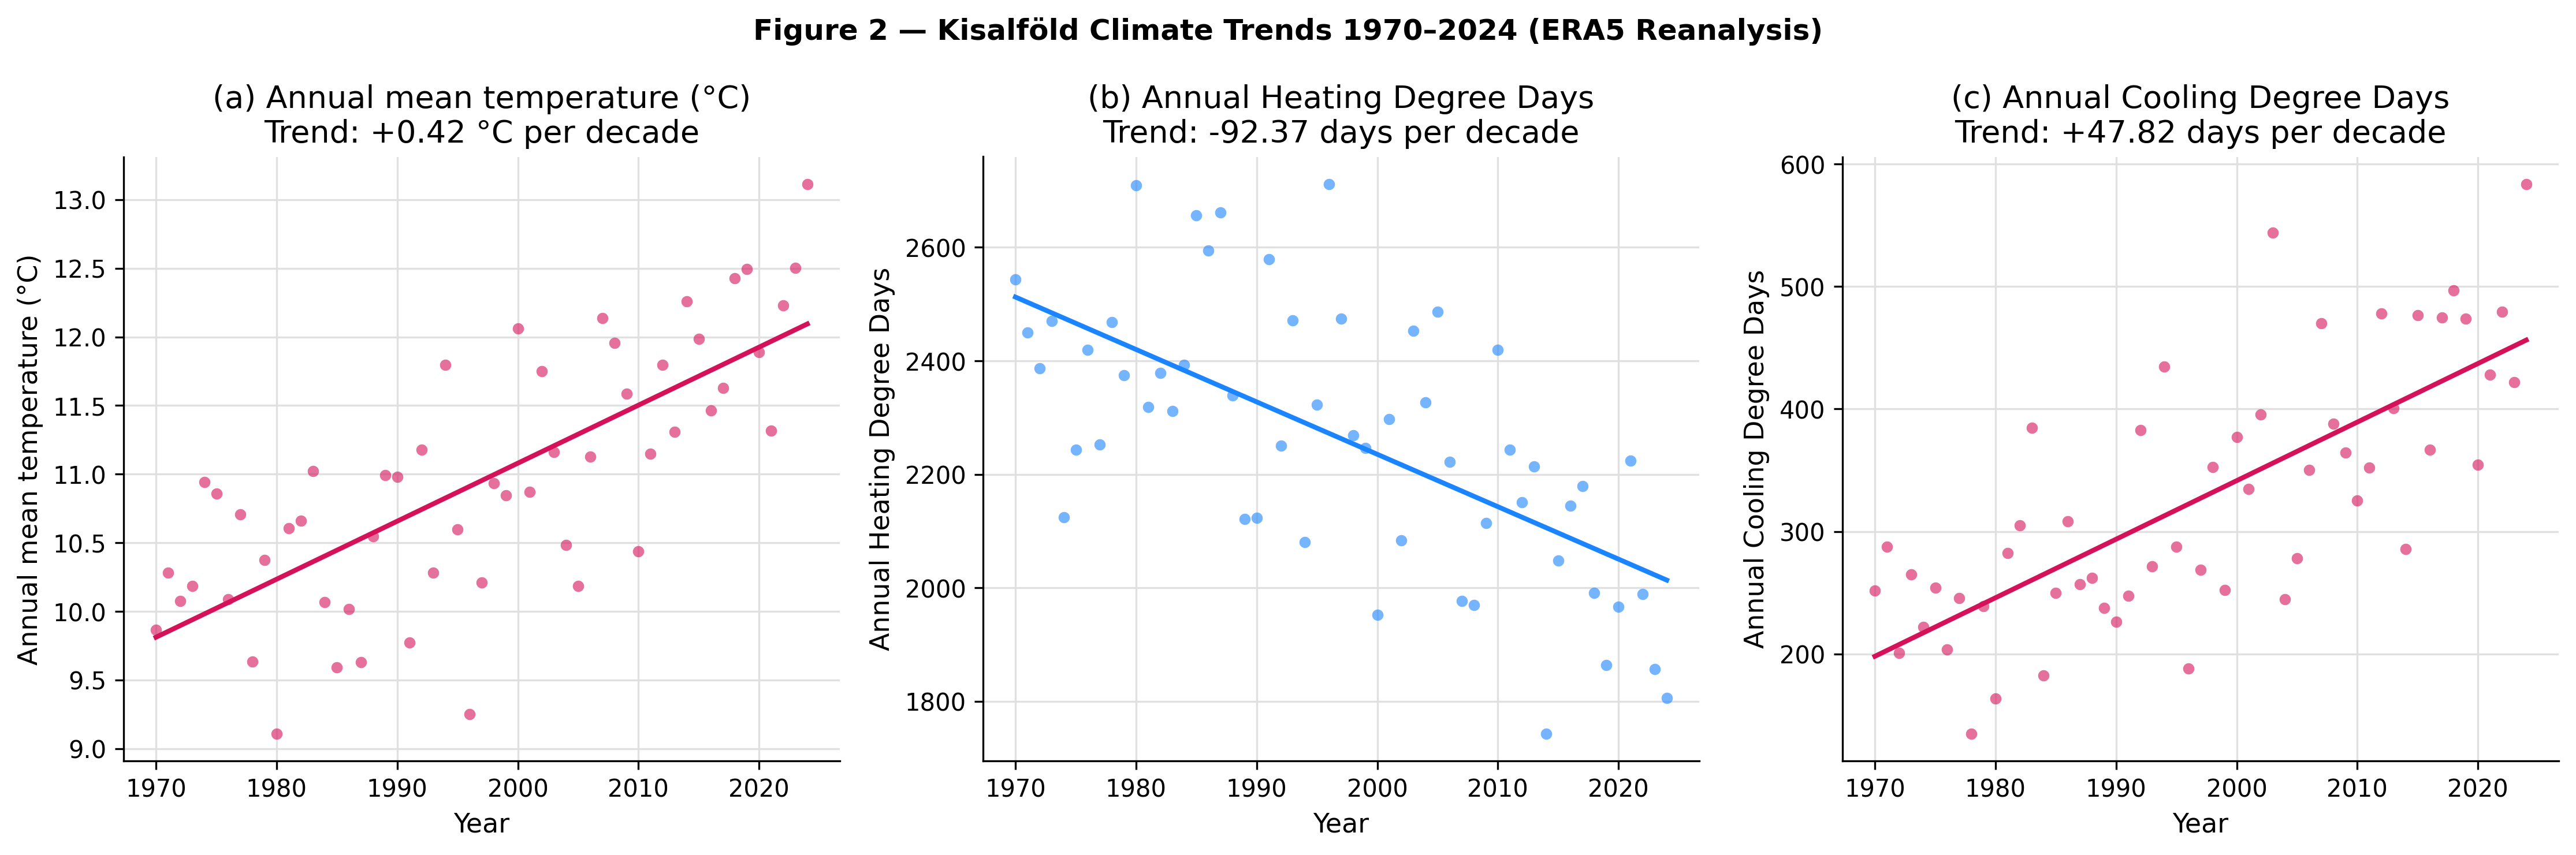
\includegraphics[width=\textwidth]{figures/fig2_climate_trends.png}
  \caption{Kisalf\"{o}ld climate trends 1970--2024 derived from ERA5
  reanalysis. (a) Annual mean surface temperature with linear trend
  ($+0.42~^\circ$C per decade). (b) Annual Heating Degree Days
  (base 15.5~$^\circ$C), trend $-92$ days per decade.
  (c) Annual Cooling Degree Days (base 18.0~$^\circ$C),
  trend $+48$ days per decade.}
  \label{fig:trends}
\end{figure}

\subsection{Temperature--Demand Relationship}
\label{sec:results_correlation}

Monthly aggregated electricity load plotted against surface temperature
reveals a clear U-shaped relationship (Figure~\ref{fig:correlation}b),
with minimum demand occurring at approximately 17~$^\circ$C. High
demand in cold winter months reflects space heating requirements, while
rising demand at temperatures above 17~$^\circ$C reflects increasing
air conditioning load. This threshold temperature is consistent with
values reported for neighbouring Central European countries
\citep{auffhammer2017}.

The XGBoost demand model trained on 2015--2021 data achieved strong
performance on the held-out 2022--2024 test set, with a coefficient of
determination $R^2 = 0.77$, root mean squared error RMSE $= 285$~MW,
and mean absolute percentage error MAPE $= 4.8$\%
(Figure~\ref{fig:model}). The model successfully captures the seasonal
demand pattern and weekly periodicity visible in the 2023 time series.

SHAP feature importance analysis (Figure~\ref{fig:shap}) reveals that
the interaction between temperature and working day patterns is the
single most influential predictor, followed by the long-term structural
demand trend and the 7-day rolling mean temperature. The dominance of
the rolling temperature term over instantaneous temperature indicates
that buildings and human behaviour exhibit significant thermal inertia.
Notably, the pre-computed HDD and CDD indices rank among the
lowest-importance features, suggesting that the XGBoost model learns
the non-linear temperature--demand relationship directly from raw
temperature variables more effectively than from aggregated indices.

\begin{figure}[htbp]
  \centering
  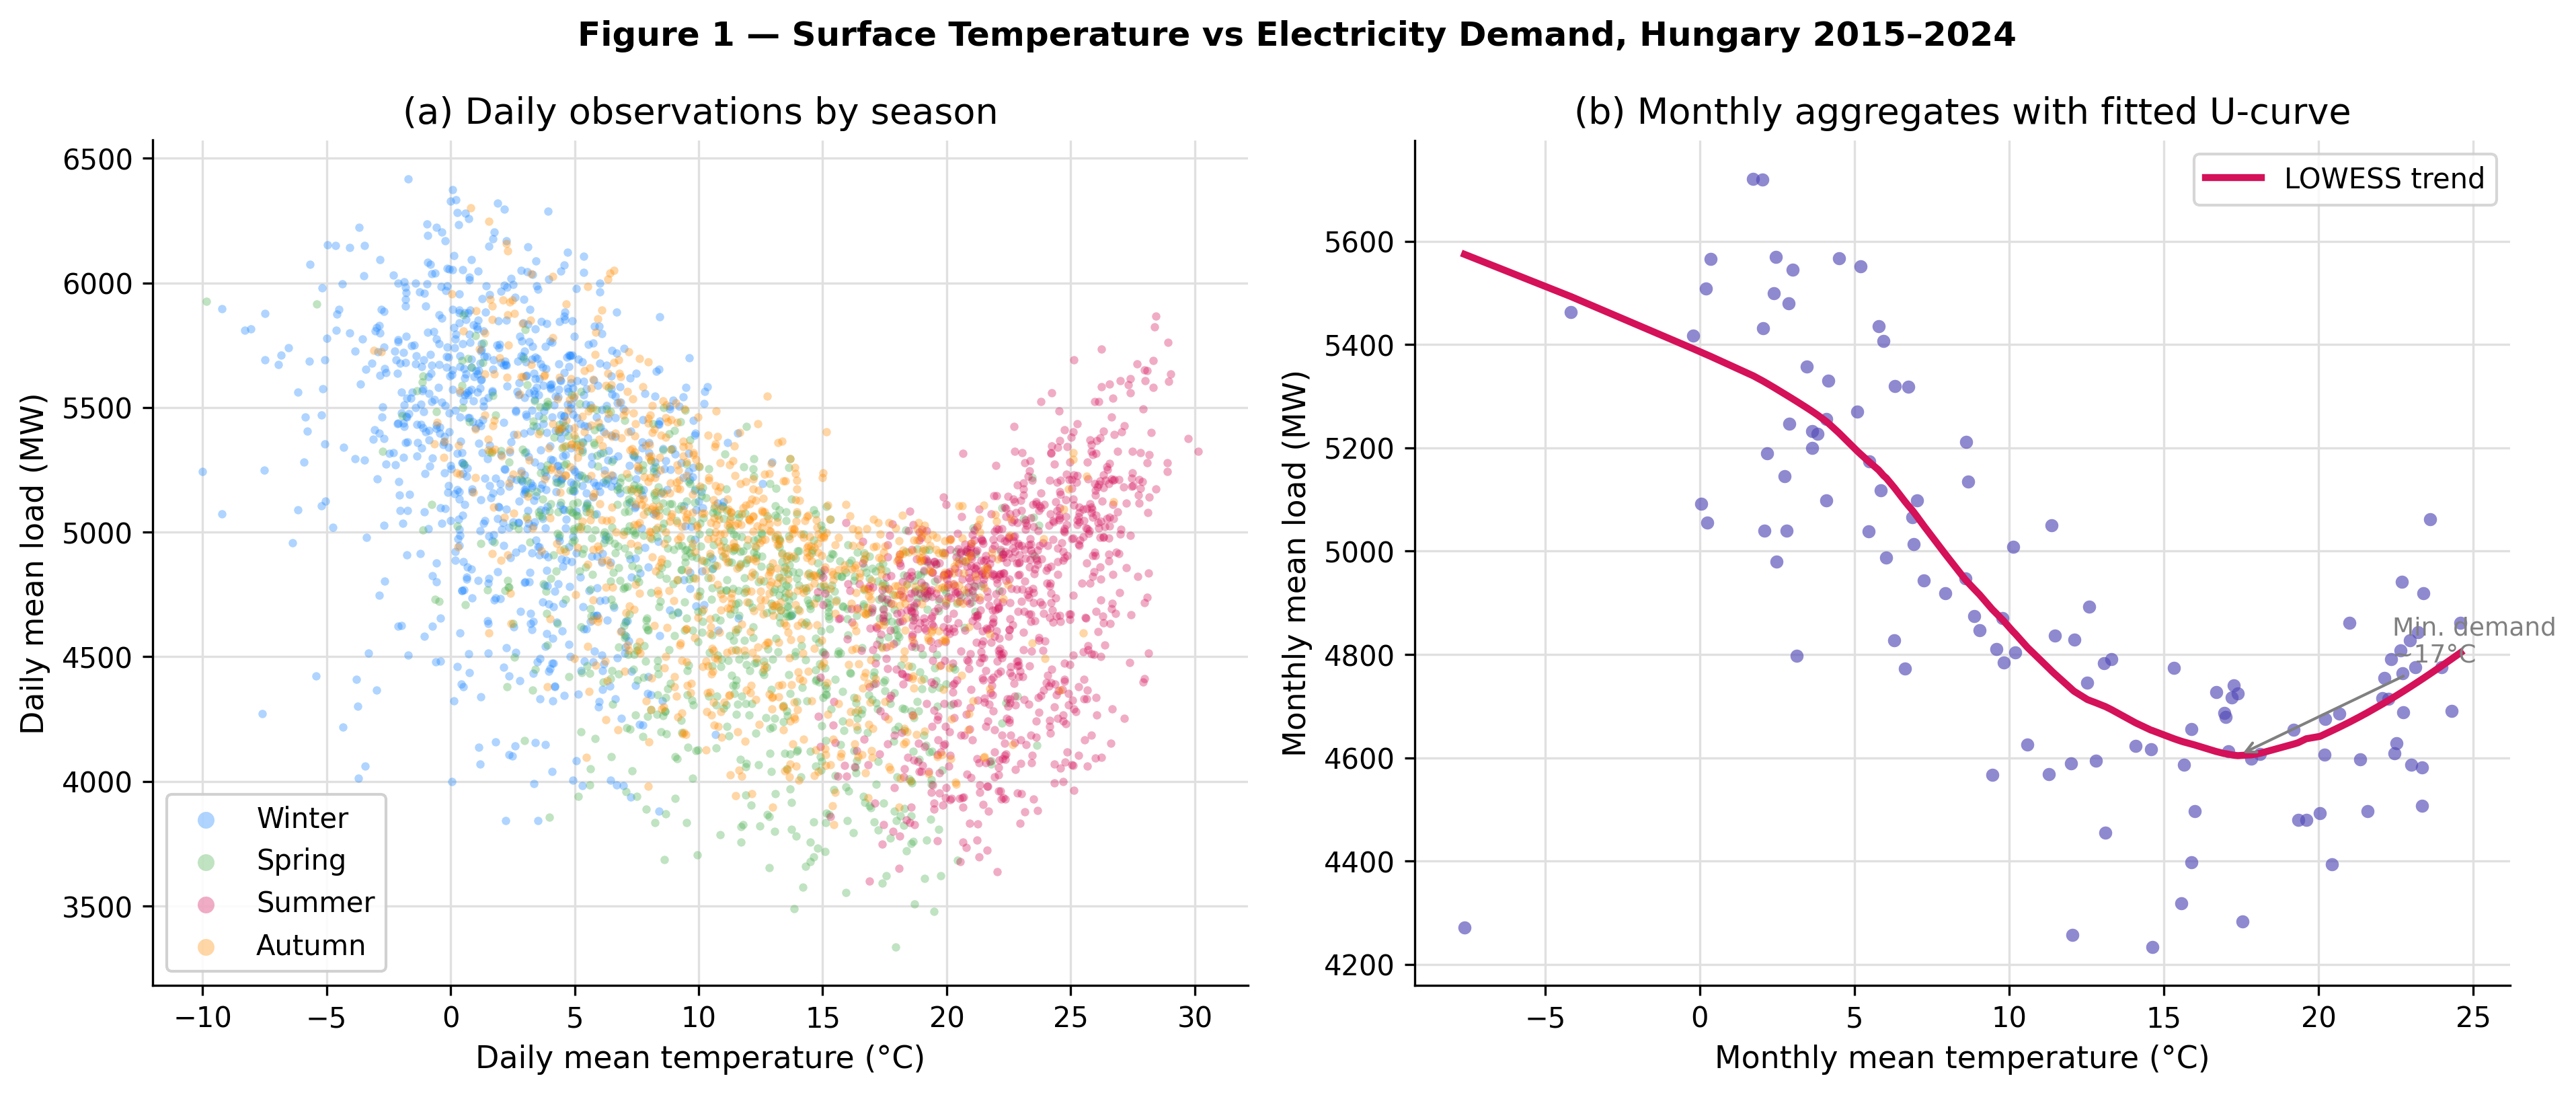
\includegraphics[width=\textwidth]{figures/fig1_temp_vs_demand.png}
  \caption{Surface temperature versus electricity demand, Hungary
  2015--2024. (a) Daily observations coloured by season.
  (b) Monthly aggregates with LOWESS trend curve, showing minimum
  demand at approximately 17~$^\circ$C.}
  \label{fig:correlation}
\end{figure}

\begin{figure}[htbp]
  \centering
  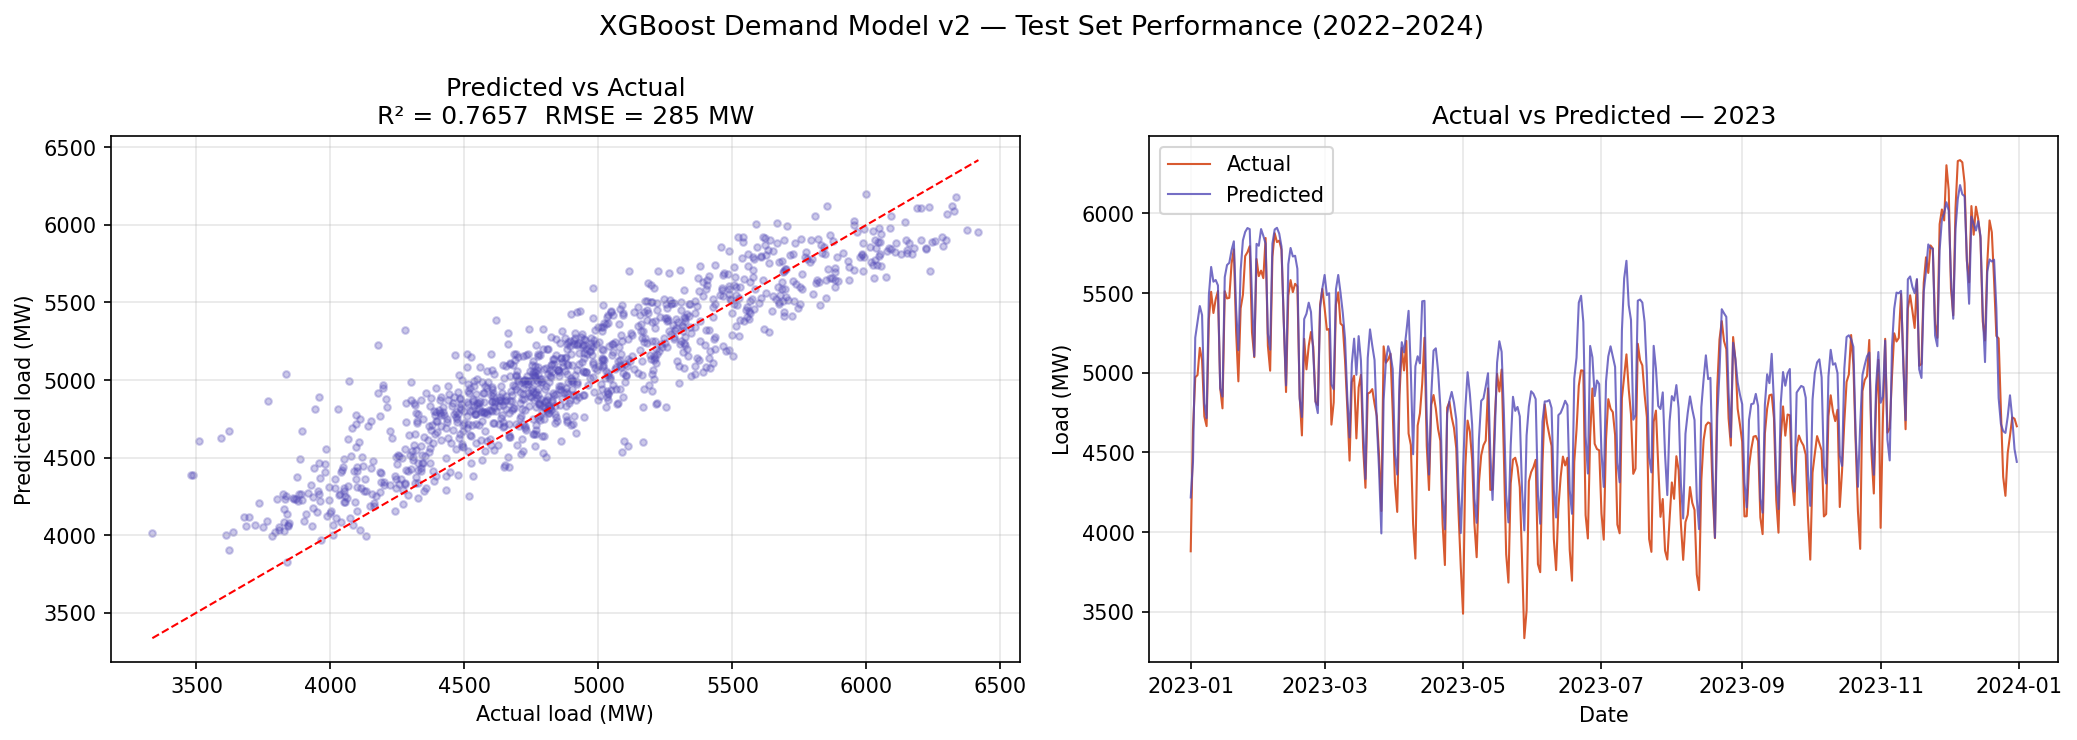
\includegraphics[width=\textwidth]{figures/fig_model_performance.png}
  \caption{XGBoost demand model performance on held-out test set
  (2022--2024). (a) Predicted versus actual daily load
  ($R^2 = 0.77$, RMSE $= 285$~MW). (b) Time series of actual and
  predicted load for 2023.}
  \label{fig:model}
\end{figure}

\begin{figure}[htbp]
  \centering
  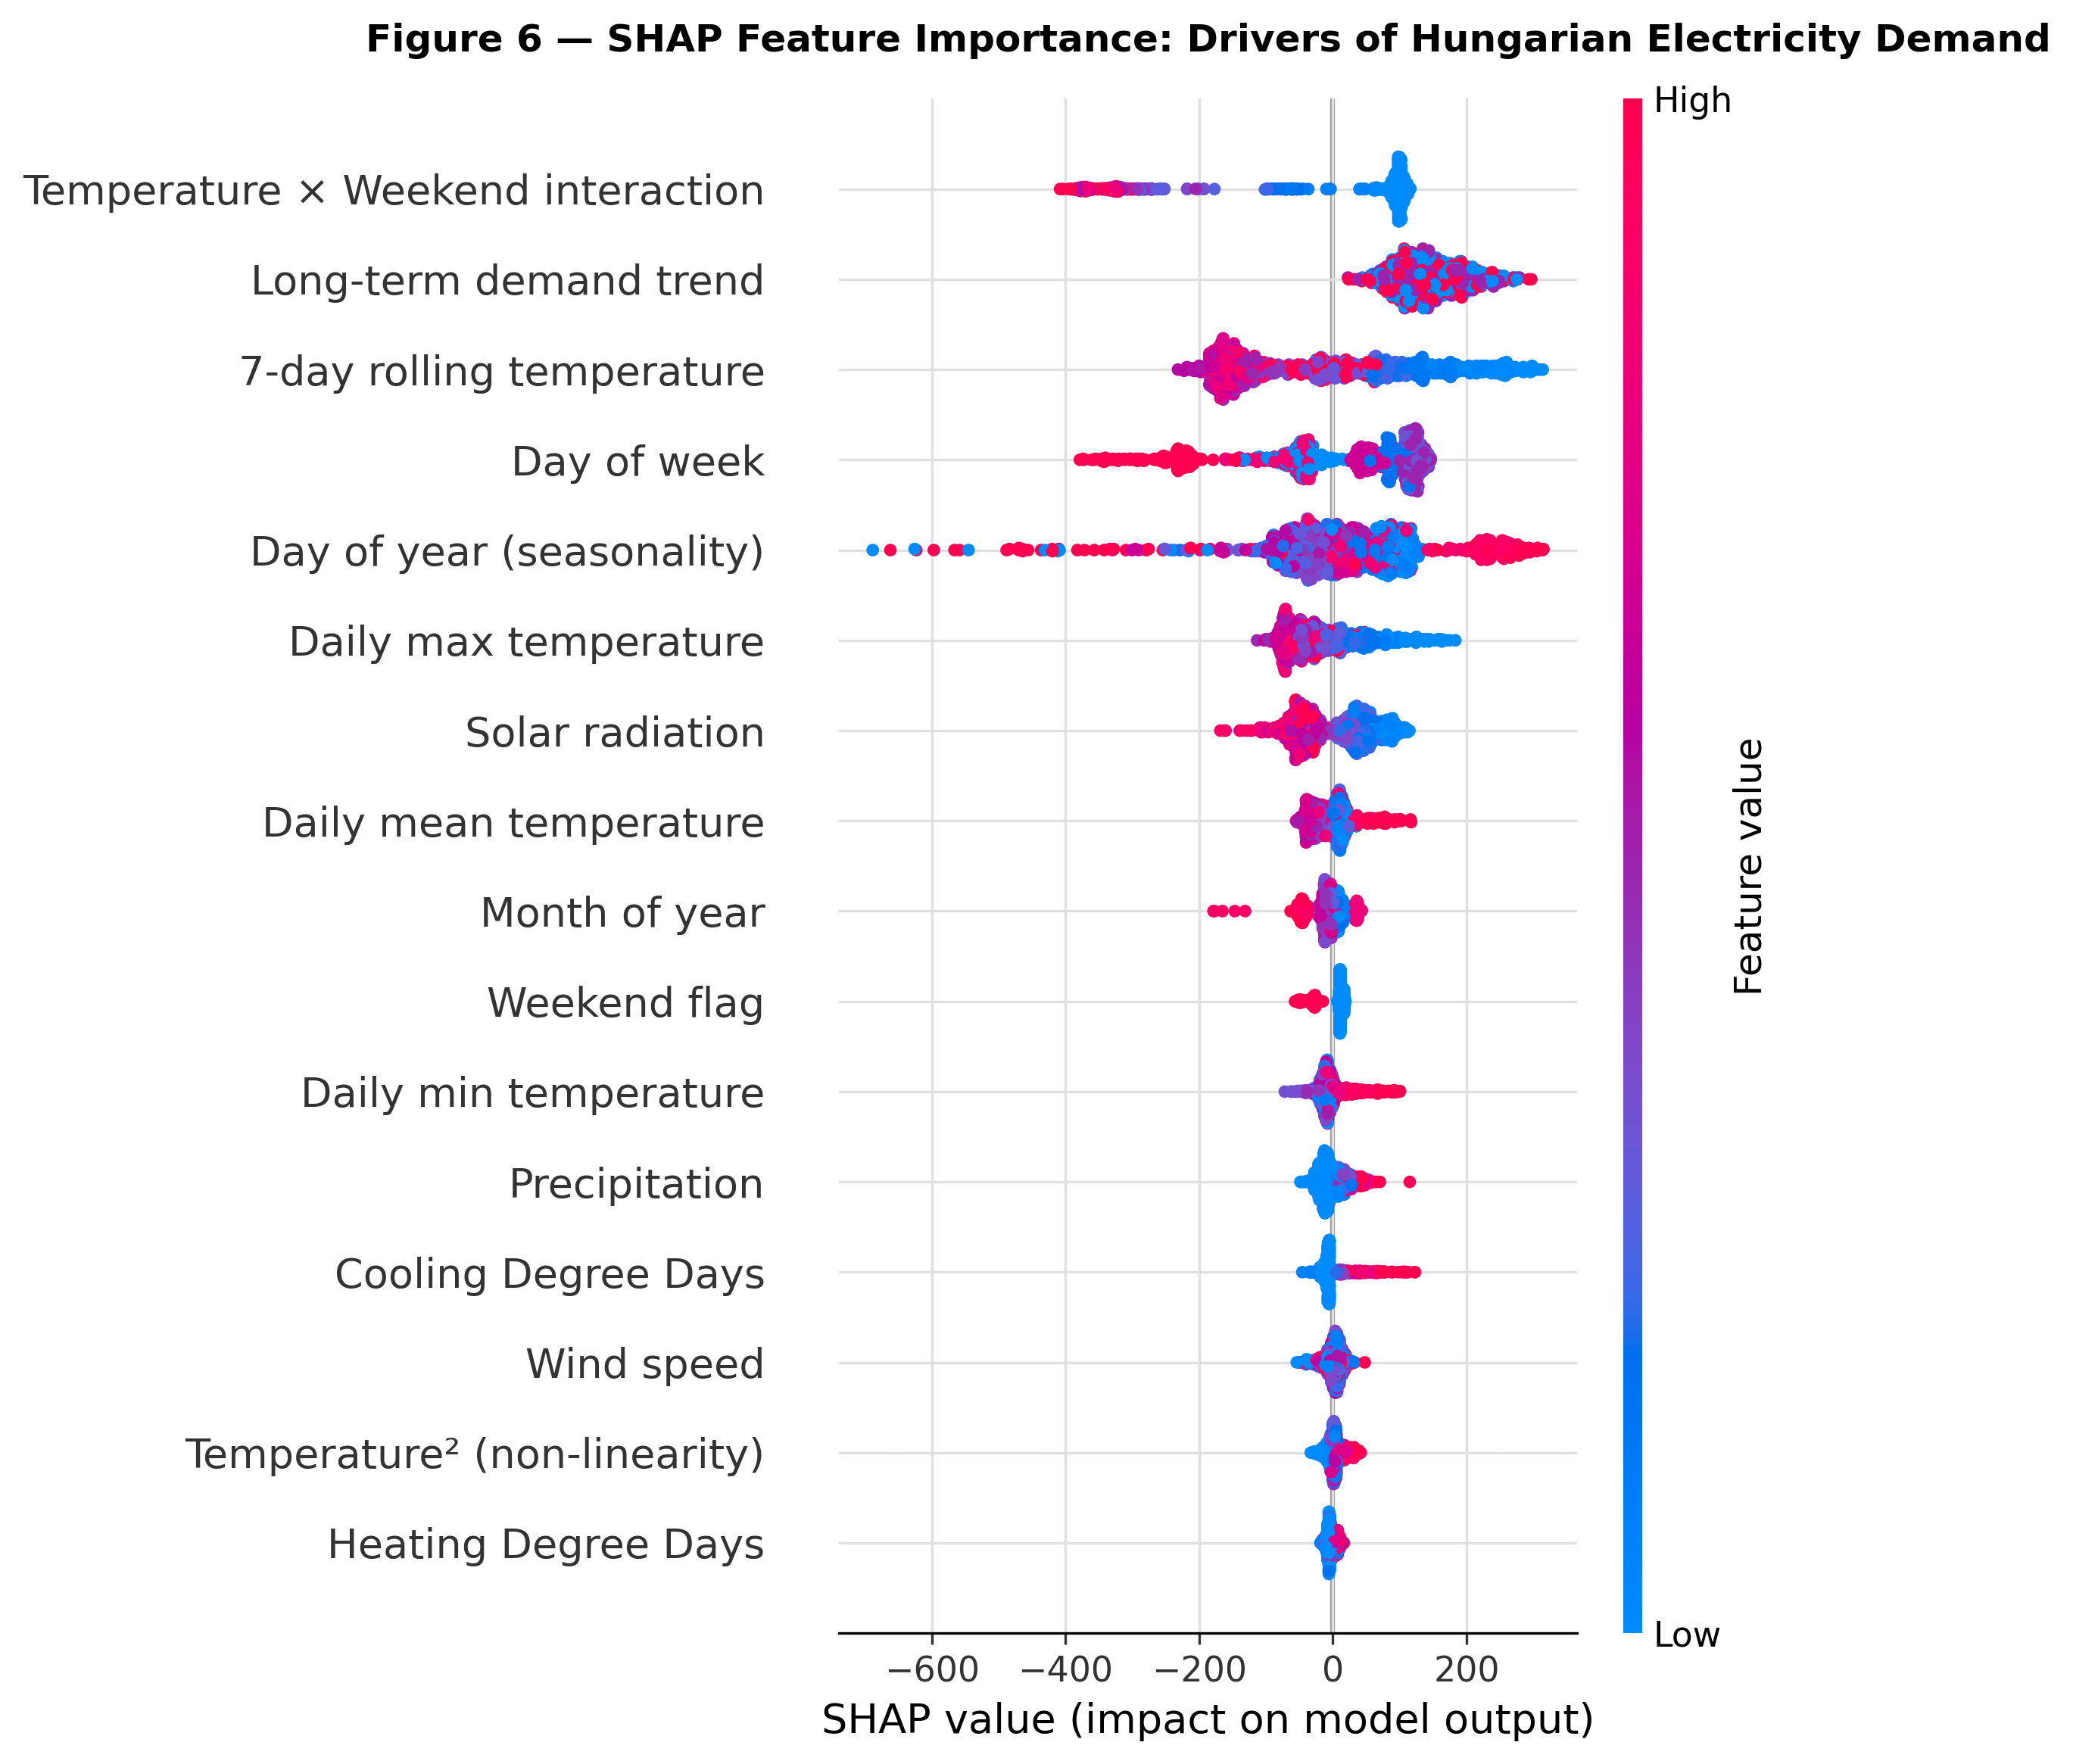
\includegraphics[width=0.85\textwidth]{figures/fig6_shap.png}
  \caption{SHAP feature importance for the XGBoost demand model.
  Each point represents one test-set observation. Colour indicates
  feature value (red = high, blue = low). Features ranked by mean
  absolute SHAP value.}
  \label{fig:shap}
\end{figure}

\subsection{Future Demand Projections}
\label{sec:results_projections}

Applying the trained demand model to IPCC AR6 temperature trajectories
yields projected demand shifts under three warming scenarios to 2100
(Figure~\ref{fig:projections}). A key finding is that the \textit{net}
climate-driven demand signal is substantially smaller than either the
heating or cooling component alone, because heating savings and cooling
gains partially offset one another.

Under SSP1-2.6, annual HDD decline by approximately 220 days by 2050
relative to 2025, while CDD increase by approximately 70 days. Under
SSP5-8.5, HDD decline by 600 days but CDD increase by 220 days, with
net demand initially falling but recovering after approximately 2065
as cooling demand begins to overtake heating savings. This crossover
point represents a structural transition from a heating-dominated to
a cooling-dominated demand profile.

By 2100 under SSP5-8.5, annual cooling degree days are projected to
reach 830 CDD yr$^{-1}$, more than four times the 1970 baseline,
while heating degree days fall below 1200 --- less than half their
1970 value.

\begin{figure}[htbp]
  \centering
  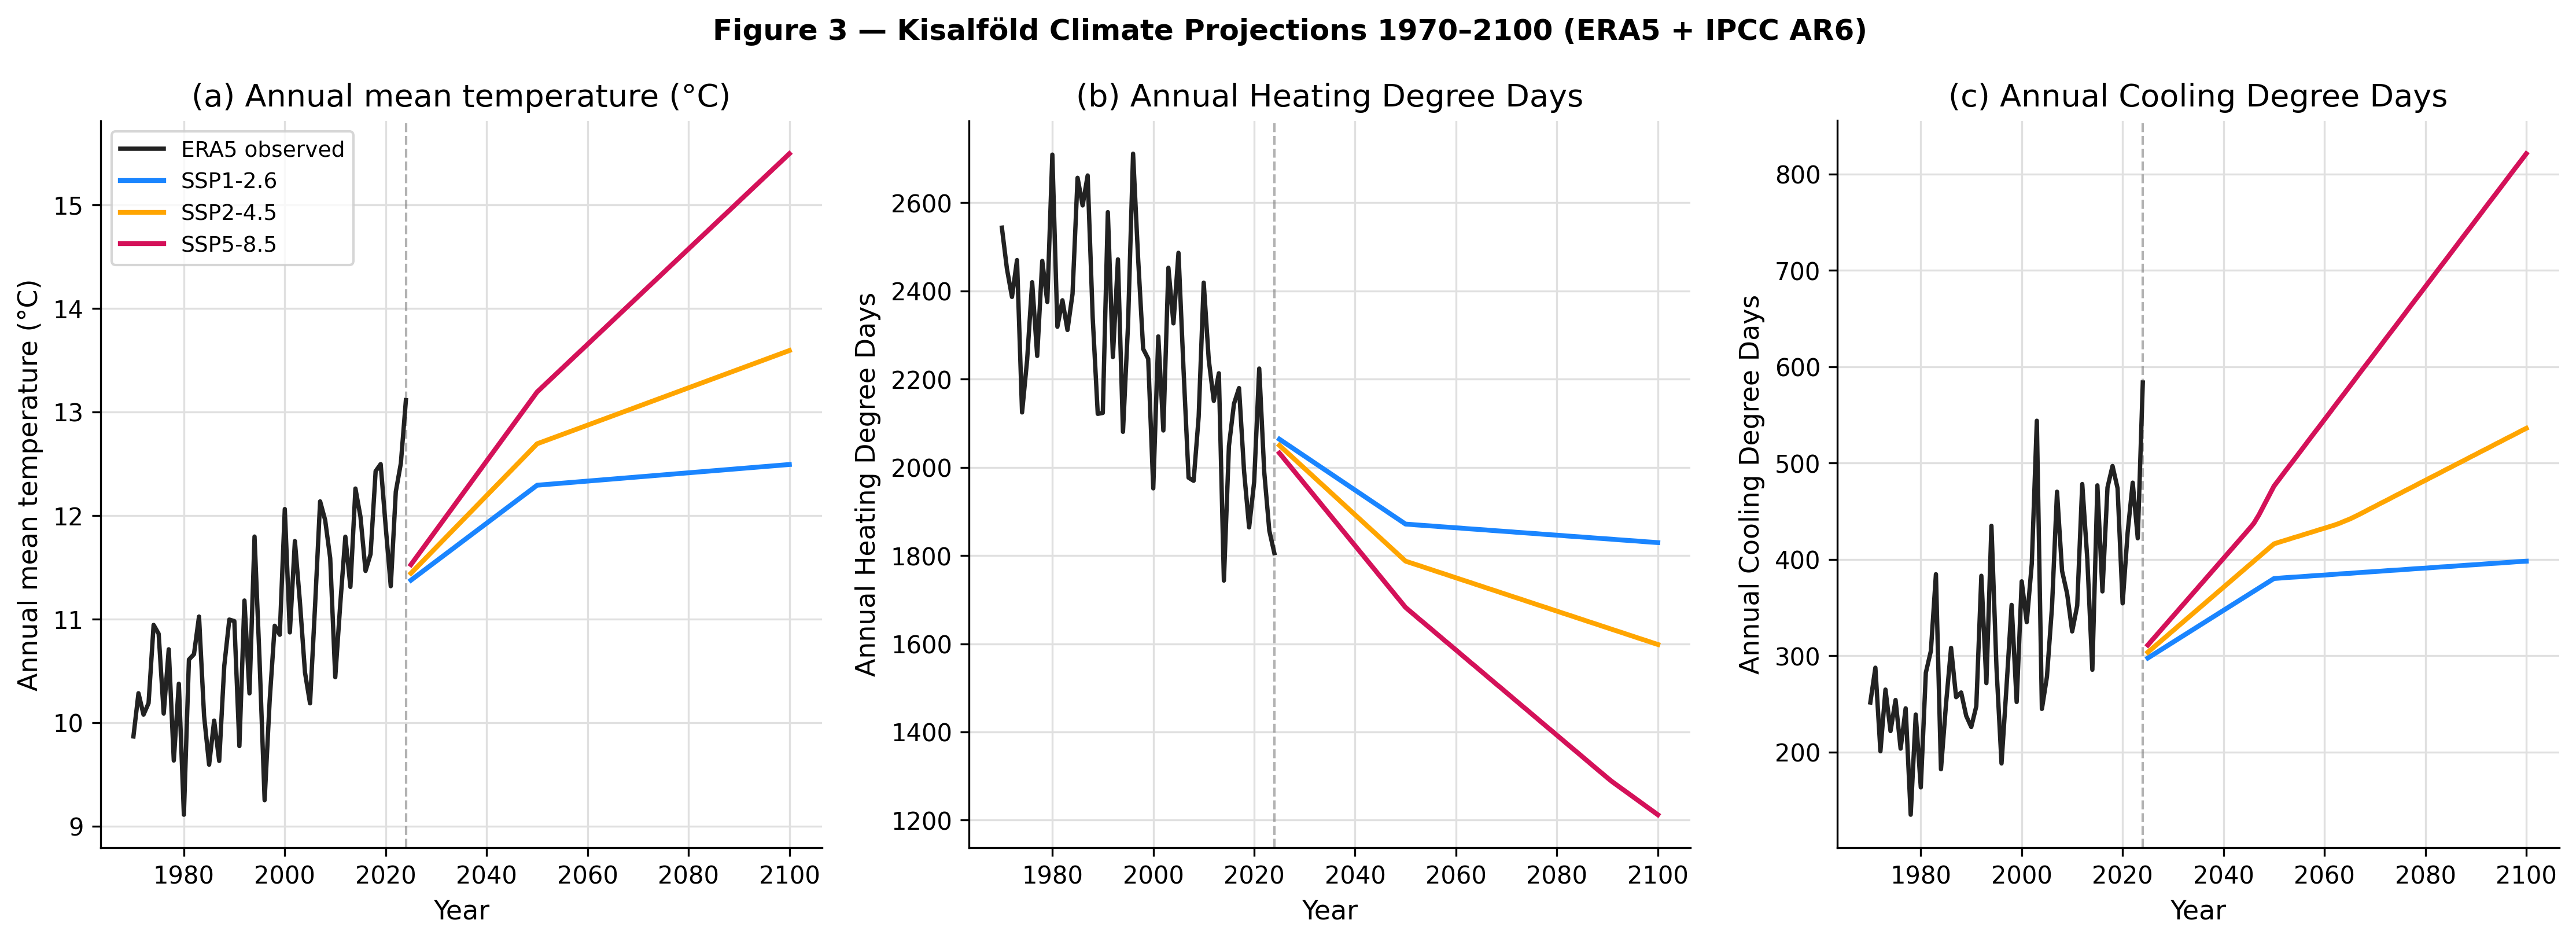
\includegraphics[width=\textwidth]{figures/fig3_projections.png}
  \caption{Kisalf\"{o}ld climate projections 1970--2100 combining
  ERA5 observations (black) and IPCC AR6 scenario trajectories.
  (a) Annual mean temperature. (b) Annual Heating Degree Days.
  (c) Annual Cooling Degree Days. Dashed vertical line marks 2024.}
  \label{fig:projections}
\end{figure}

\begin{figure}[htbp]
  \centering
  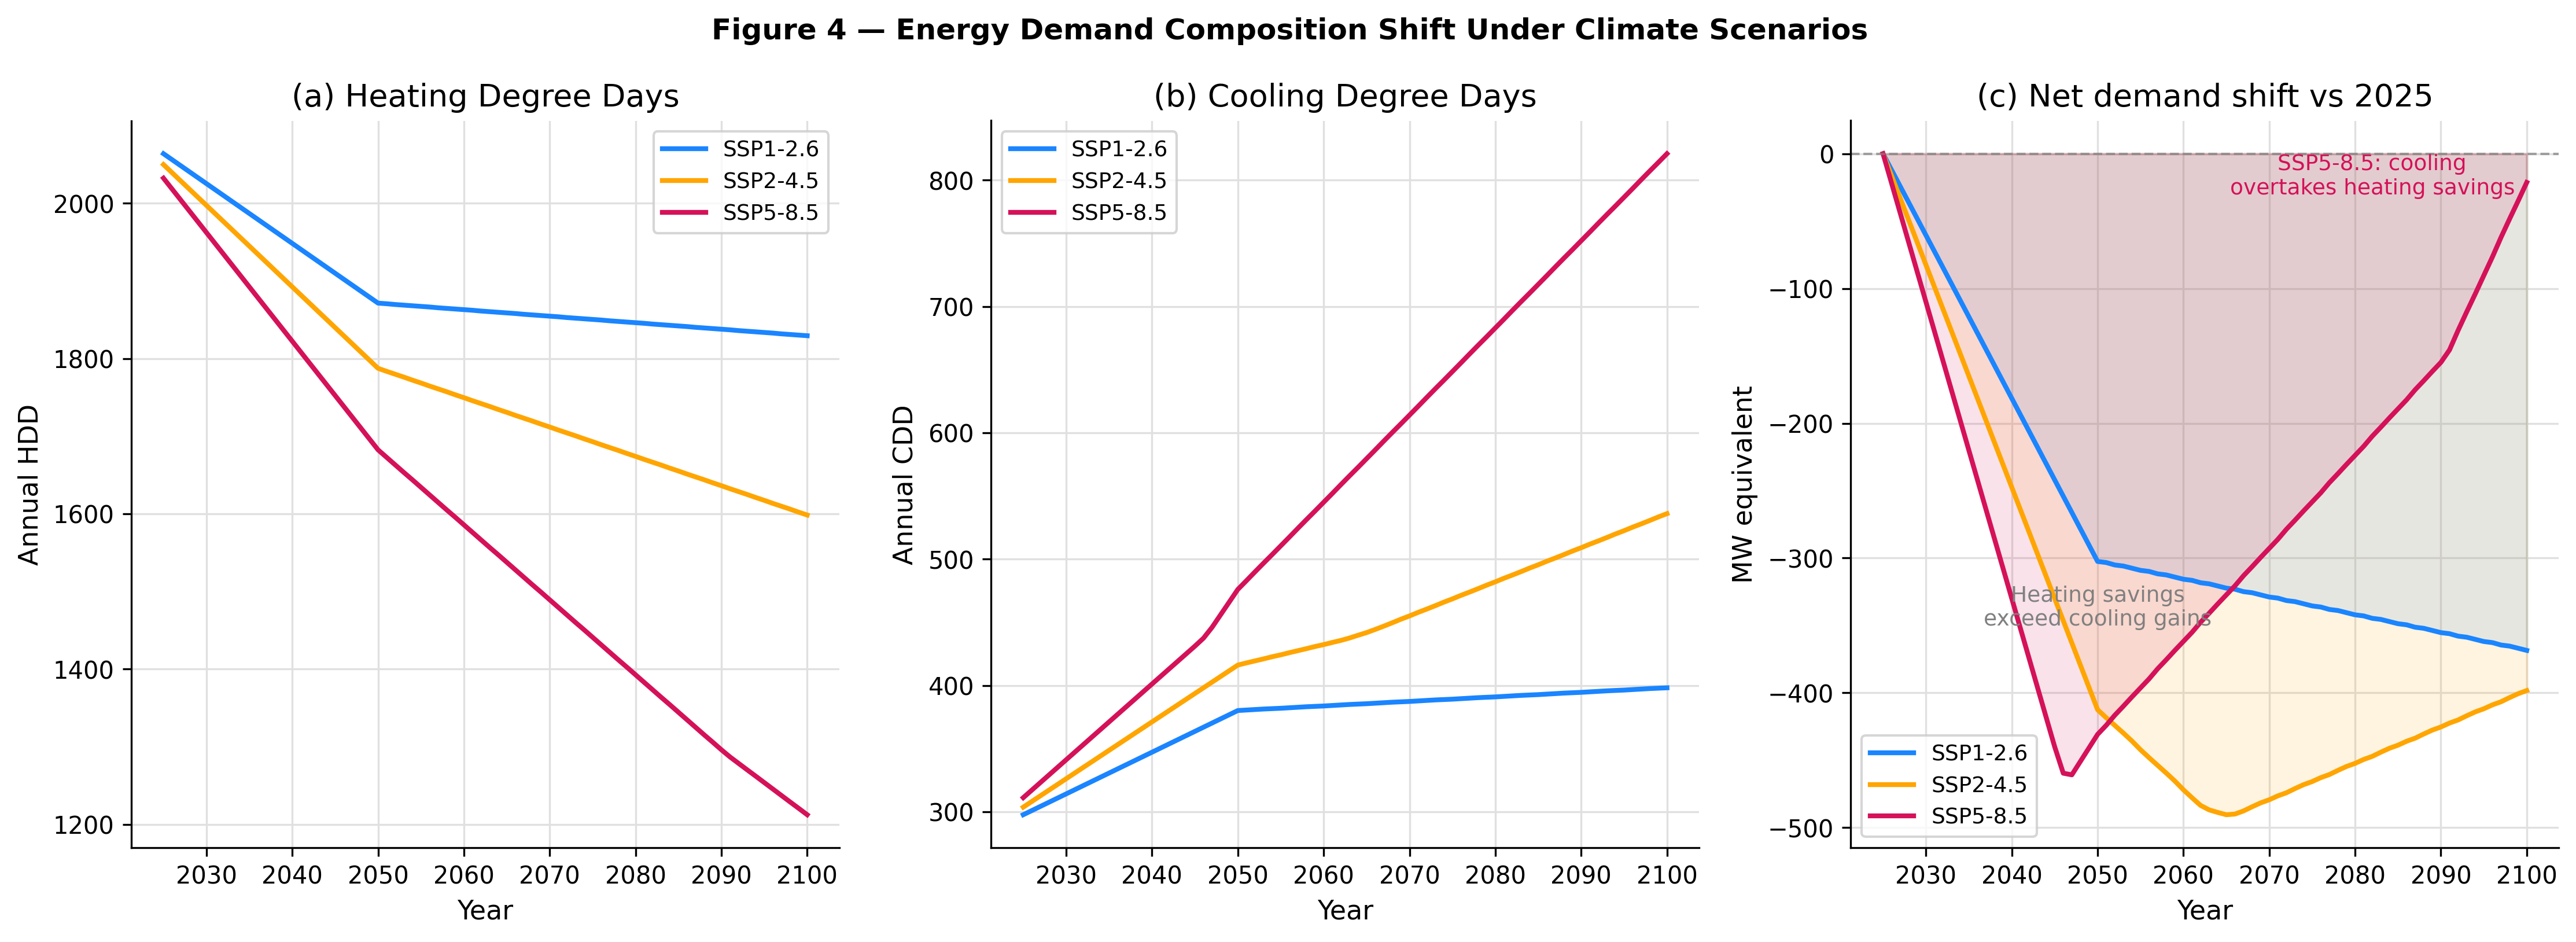
\includegraphics[width=\textwidth]{figures/fig4_demand_composition.png}
  \caption{Energy demand composition shift under climate scenarios.
  (a) Annual Heating Degree Days. (b) Annual Cooling Degree Days.
  (c) Net demand shift relative to 2025 baseline (MW equivalent),
  showing the crossover point under SSP5-8.5 around 2065.}
  \label{fig:composition}
\end{figure}

\subsection{Infrastructure Loss Amplification}
\label{sec:results_losses}

Using the ENTSO-E baseline transmission loss rate of 6.5\% and a
temperature sensitivity of 0.4 percentage points per degree Celsius
of warming above the 1991--2020 baseline, we estimate that the grid
transmission loss rate increases to 6.8\% under SSP1-2.6, 7.3\%
under SSP2-4.5, and 8.1\% under SSP5-8.5 by 2100
(Figure~\ref{fig:losses}a).

The resulting wasted generation increases from approximately 350~MW
at the 2025 baseline to 370~MW under SSP1-2.6, 400~MW under SSP2-4.5,
and 450~MW under SSP5-8.5 by 2100 (Figure~\ref{fig:losses}b). Under
the high-emissions scenario, this represents an additional ~100~MW of
continuously wasted generation capacity attributable solely to
temperature-driven resistance increases.

\begin{figure}[htbp]
  \centering
  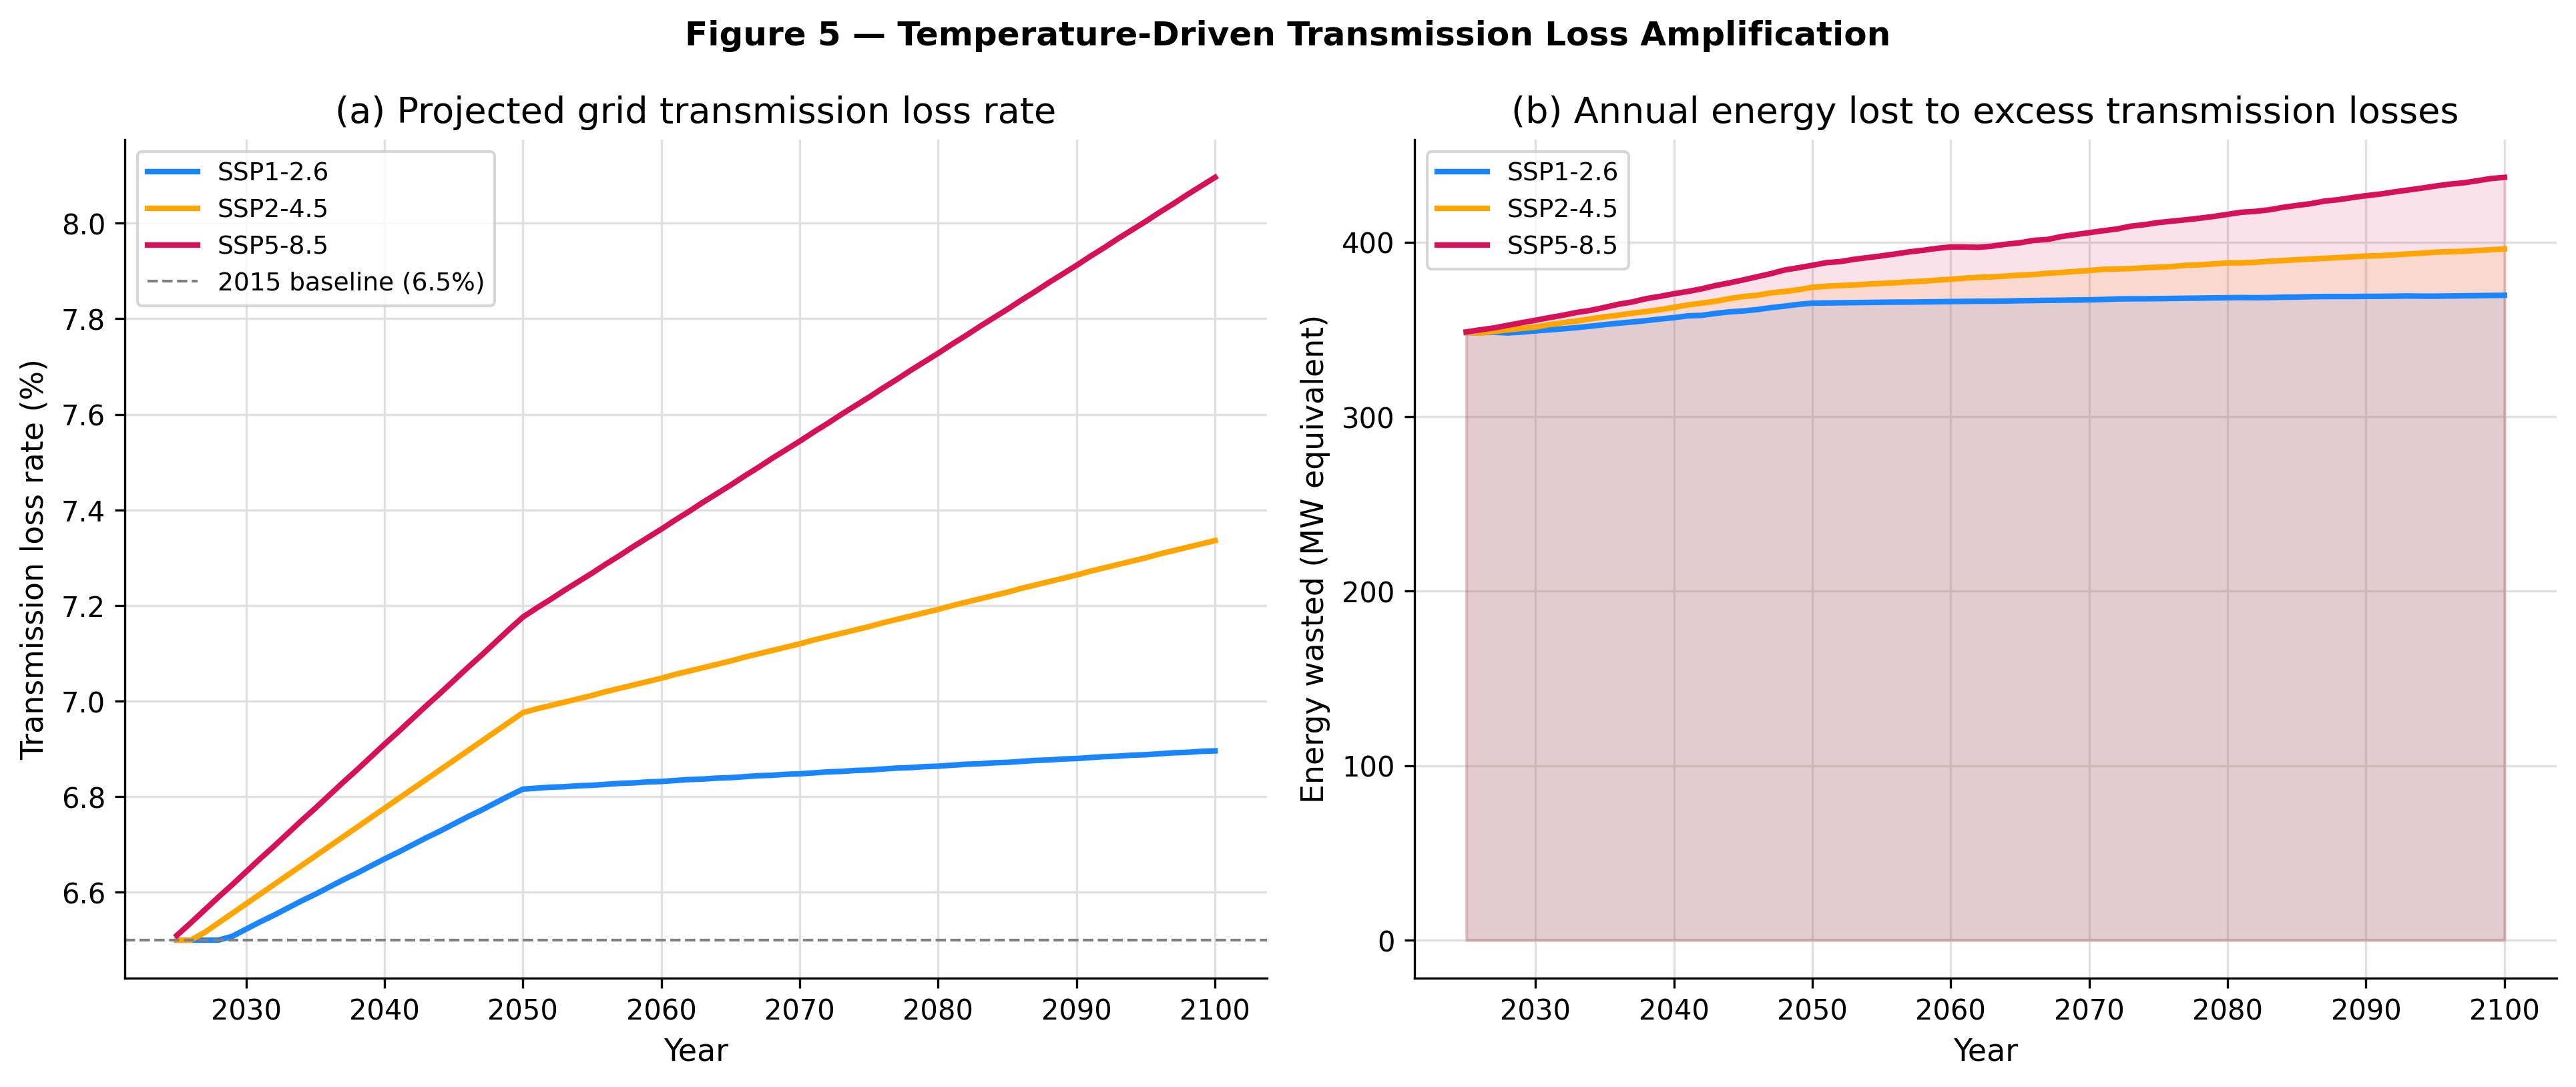
\includegraphics[width=\textwidth]{figures/fig5_loss_amplification.png}
  \caption{Temperature-driven transmission loss amplification under
  three warming scenarios. (a) Projected grid transmission loss rate
  (\%). Dashed line shows 2015 baseline (6.5\%).
  (b) Annual energy lost to excess transmission losses (MW equivalent).}
  \label{fig:losses}
\end{figure}

% ── 5. Discussion ────────────────────────────────────────────────────────────
\section{Discussion}
\label{sec:discussion}

\subsection{Demand Restructuring, Not Just Demand Growth}
\label{sec:disc_restructuring}

The central finding of this study is that climate change does not
simply increase Hungary's electricity demand --- it fundamentally
restructures it. Under moderate and optimistic warming scenarios,
net climate-driven demand may actually decline through mid-century
as heating savings outpace cooling gains. However, this apparent
benefit masks a more challenging infrastructure reality: the
\textit{timing} and \textit{seasonality} of demand shifts
dramatically. Hungary's grid was designed for winter peaks driven
by heating demand. A transition to summer-peak demand driven by
air conditioning requires different generation capacity, different
storage solutions, and different grid management strategies ---
even if the annual total demand remains similar.

The crossover point identified under SSP5-8.5, where cooling demand
overtakes heating savings around 2065, represents a critical planning
horizon for Hungarian energy infrastructure. Investment decisions made
today will determine whether this transition is managed smoothly or
results in systemic stress.

\subsection{The Compounding Loss Effect}
\label{sec:disc_losses}

The transmission loss amplification effect represents a largely
overlooked dimension of climate--energy interactions. While the
absolute magnitude (up to ~100~MW by 2100 under SSP5-8.5) is modest
relative to Hungary's total generation capacity of approximately 10~GW,
the effect concentrates on the hottest days when the grid is already
under maximum stress from peak cooling demand. The combination of peak
demand and peak losses on the same days represents a compounding risk
not captured by annual average analyses.

\subsection{Limitations and Uncertainties}
\label{sec:disc_limitations}

Several limitations should be noted. First, the demand model is trained
on national Hungarian load data rather than Kisalf\"{o}ld-specific
consumption, as sub-regional load data are not publicly available.
Second, the IPCC AR6 warming deltas represent multi-model ensemble best
estimates and do not capture the full uncertainty range of individual
model projections. Third, the transmission loss sensitivity parameter
is derived from European aggregate data and may not accurately represent
Hungary's specific grid infrastructure. Fourth, the model does not
account for future changes in building stock, appliance efficiency,
electrification of heating and transport, or demand-side interventions.

Future work should incorporate sub-regional load data, apply
bias-corrected individual CMIP6 model runs to quantify projection
uncertainty, and extend the framework to explicitly model the
electrification transition expected under Hungary's National Energy
and Climate Plan.

\subsection{Policy Implications}
\label{sec:disc_policy}

The findings carry several implications for Hungarian energy policy.
The projected shift toward summer-peak demand argues for accelerated
investment in solar generation capacity. Grid reinforcement and
deployment of high-temperature-rated conductors can directly mitigate
the transmission loss amplification effect. Demand-side cooling
efficiency standards would reduce the cooling demand growth underlying
both the demand shift and the loss amplification. Finally, the study
underscores the importance of scenario-specific infrastructure planning:
the difference between SSP1-2.6 and SSP5-8.5 outcomes by 2100 is
structural, representing fundamentally different energy systems
requiring fundamentally different infrastructure.

% ── 6. Conclusion ────────────────────────────────────────────────────────────
\section{Conclusion}
\label{sec:conclusion}

This study has quantified the historical and projected climate-driven
shifts in energy demand for the Kisalf\"{o}ld region of Hungary using
54 years of ERA5 reanalysis, 16 years of upper-air sounding data, and
10 years of national grid load records. Key findings are: (1) the region
has warmed by $+0.42~^\circ$C per decade since 1970, with cooling degree
days tripling and heating degree days declining by 20\%; (2) a gradient-
boosted demand model ($R^2 = 0.77$) reveals that thermal inertia and
temperature--weekday interactions are the primary climate drivers of
demand; (3) net demand restructuring rather than net demand growth is
the dominant climate signal, with cooling overtaking heating under
high-emissions scenarios around 2065; and (4) temperature-driven
transmission losses add up to 100~MW of wasted generation capacity by
2100 under SSP5-8.5, a compounding burden concentrated on peak demand
days. These findings argue for solar-oriented generation investment,
grid reinforcement, and scenario-specific infrastructure planning in
Hungary's energy transition.

% ── Acknowledgements ─────────────────────────────────────────────────────────
\section*{Acknowledgements}

ERA5 data were obtained from the Copernicus Climate Change Service.
ENTSO-E Transparency Platform data are used under their open data
policy. Upper-air sounding data were obtained from the University of
Wyoming upper-air archive. The author thanks the open-source communities
behind Python, XGBoost, and the scientific Python ecosystem.

% ── Data Availability ────────────────────────────────────────────────────────
\section*{Data and Code Availability}

All code, processed datasets, and an interactive visualisation are
publicly available at:\\
\url{https://github.com/Zoomb-o/kisalfold-climate-energy}

The interactive PWA is accessible at:\\
\url{https://zoomb-o.github.io/kisalfold-climate-energy}

% ── References ───────────────────────────────────────────────────────────────
\bibliographystyle{apalike}
\bibliography{references}

% ── Appendix ─────────────────────────────────────────────────────────────────
\appendix

\section{Sounding Station Metadata}
\label{app:soundings}

Upper-air sounding data were obtained from WMO station 12843
(Budapest/Pestszentl\H{o}rinc), coordinates $47.43^\circ$N,
$19.18^\circ$E, elevation 139~m. Data span January 2010 to May 2026,
with 00Z and 12Z launches daily. Mean data availability was 1.84
soundings per day (92\% of possible observations), with missing data
attributed to server availability at the University of Wyoming archive.

\section{Model Hyperparameters}
\label{app:hyperparams}

\begin{table}[htbp]
  \centering
  \caption{XGBoost hyperparameters used in the final demand model.}
  \begin{tabular}{ll}
    \toprule
    Parameter & Value \\
    \midrule
    n\_estimators & 1000 \\
    learning\_rate & 0.03 \\
    max\_depth & 5 \\
    subsample & 0.8 \\
    colsample\_bytree & 0.8 \\
    min\_child\_weight & 3 \\
    random\_state & 42 \\
    \bottomrule
  \end{tabular}
  \label{tab:hyperparams}
\end{table}

\end{document}